\documentclass{article}
\usepackage{graphicx} % Required for inserting images

\title{File Transfer Protocol}
\author{Do Tuan Dung BI12-104}
\date{\today}

\begin{document}

\maketitle

\begin{abstract}
This report documents the implementation of a file transfer system using sockets in C. The system enables a client to send a file to a server over a network connection. The report details the system overview, implementation details of the server and client code, and provides relevant code snippets for illustration.
\end{abstract}

\section{Introduction}

This report describes the development of a file transfer system using sockets in C. The project allows a client to send a file to a server on the same network, facilitating data exchange between machines.

\section{System Overview:}
The system consists of two main components:

- Server: The server listens for incoming connections on a predefined port. Once a client connects, the server receives the filename and file data from the client and stores the received data in a designated file.

- Client: The client initiates a connection to the server's IP address and port. After establishing the connection, the client sends the filename and file data to the server. Finally, the client receives feedback on the transfer status from the server.
\section{Implementation Details:}
\subsection{Client:}
The client establishes a connection, sends the filename, and transmits the file data. Here is the "client.c" file:
\begin{verbatim}
    #include <sys/socket.h>
    #include <netinet/in.h>
    #include <stdio.h>
    #include <stdlib.h>
    #include <string.h>
    #include <unistd.h>
    #include <arpa/inet.h>
    
    #define BUFFER_SIZE 1024
    
    int main() {
      int sockfd;
      struct sockaddr_in server_addr;
      char buffer[BUFFER_SIZE];
      int recv_len;
      char filename[BUFFER_SIZE];
      FILE *fp;
    
      memset(buffer, 0, sizeof(buffer));
      memset(&server_addr, 0, sizeof(server_addr));
    
      sockfd = socket(AF_INET, SOCK_STREAM, 0);
      if (sockfd == -1) {
        perror("socket");
        exit(1);
      }
    
      server_addr.sin_family = AF_INET;
      server_addr.sin_addr.s_addr = inet_addr("127.0.0.1");
      server_addr.sin_port = htons(5000);
    
      if (connect(sockfd, (struct sockaddr*)&server_addr, sizeof(server_addr)) < 0) {
        perror("connect");
        exit(1);
      }
    
      printf("Enter the filename to send: ");
      fgets(filename, BUFFER_SIZE, stdin);
      filename[strcspn(filename, "\n")] = 0; 
    
      send(sockfd, filename, strlen(filename), 0);
    
      fp = fopen("received_file", "wb");
      if (fp == NULL) {
        perror("fopen");
        close(sockfd);
        exit(1);
      }
    
      while ((recv_len = recv(sockfd, buffer, BUFFER_SIZE, 0)) > 0) {
        fwrite(buffer, sizeof(char), recv_len, fp);
        if (recv_len < BUFFER_SIZE) {
          break; 
        }
      }
    
      if (recv_len < 0) {
        perror("recv");
      }
    
      fclose(fp);
      close(sockfd);
    
      if (recv_len == 0) {
        printf("File sent successfully!\n");
      } else {
        printf("Error receiving file.\n");
      }
    
      return 0;
    }

\end{verbatim}

\subsection{Server:}
The server awaits client connections and accepts file transfers. Here is the "server.c" file:
\begin{verbatim}
    #include <sys/socket.h>
    #include <netinet/in.h>
    #include <stdio.h>
    #include <stdlib.h>
    #include <string.h>
    #include <unistd.h>
    #include <arpa/inet.h>
    #include <time.h>
    #include <sys/types.h>
    #include <errno.h>
    #include <fcntl.h>
    
    #define BUFFER_SIZE 1024
    
    int main(){
      int listenfd = -1;
      int connfd = -1;
      struct sockaddr_in server_addr;
      char buffer[BUFFER_SIZE];
      int file_fd;
      int bytes_read;
    
      memset(buffer, 0, sizeof(buffer));
      memset(&server_addr, 0, sizeof(server_addr));
    
      listenfd = socket(AF_INET, SOCK_STREAM, 0);
      server_addr.sin_family = AF_INET;
      server_addr.sin_addr.s_addr = inet_addr("127.0.0.1");
      server_addr.sin_port = htons(5000);
    
      bind(listenfd, (struct sockaddr*)&server_addr, sizeof(server_addr));
      listen(listenfd, 10);
    
      while(1) {
        connfd = accept(listenfd, (struct sockaddr*)NULL, NULL);
        if (connfd < 0) {
          perror("accept");
          continue;
        }
    
        int recv_len = recv(connfd, buffer, BUFFER_SIZE - 1, 0);
        if (recv_len > 0) {
          buffer[recv_len] = '\0';
          printf("Requested file: %s\n", buffer);
        } else {
          perror("recv");
          close(connfd);
          continue;
        }
    
        file_fd = open(buffer, O_RDONLY);
        if (file_fd < 0) {
          perror("open");
          send(connfd, "Error opening file", strlen("Error opening file"), 0);
          close(connfd);
          continue;
        }
    
        while ((bytes_read = read(file_fd, buffer, BUFFER_SIZE)) > 0) {
          send(connfd, buffer, bytes_read, 0);
        }
    
        close(file_fd);
        close(connfd);
      }
      close(listenfd);
    }

\end{verbatim}
\section{Result:}
Here is the result after compile:
\begin{figure}[h!]
    \centering
    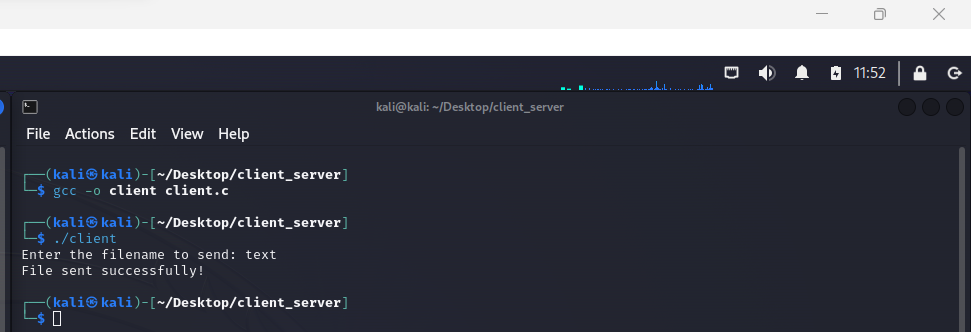
\includegraphics[scale=0.5]{client.png}
    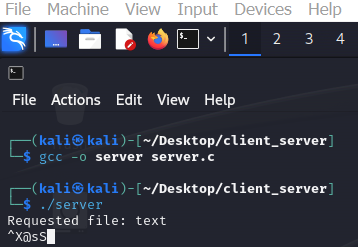
\includegraphics[scale=0.5]{server.png}
    \caption{TCP file transfer flowchart}
    \label{fig:enter-label}
\end{figure}
\end{document}

